\documentclass[../main.tex]{subfiles}
\graphicspath{ {../../results/} }

\usepackage{caption}
\usepackage{subcaption}

\begin{document}
    \justify
    \section{Badania wpływu wartości wag początkowych na szybkość uczenia}
    \paragraph{}
    Badanie ma na celu zbadanie wpływu wartości wag początkowych na działanie perceptronu prostego oraz Adaline. Badania przeprowadzone zostały dla unipolarnej funkcji aktywacji oraz unipolarnego zbioru uczącego. Wykorzystano współczynnik uczenia a = 0.05.
    
    \paragraph{}
    Zbadano natomiast następujące przedziały:
    \begin{itemize}
     \item (-1, 1)
     \item (-0.8,  0.8)
     \item (-0.6, 0.6)
     \item (-0.4, 0.4)
     \item (-0.2, 0.2)
     \item (-0.05, 0.05)
     \item (0, 0)
    \end{itemize}
    
    \paragraph{}
    Tak jak zostało to wcześniej wspomniane, prezentowane wyniki są wartościami uśrednionymi, \\hline
    uzyskanymi w skutek wielokrotnego uruchomienia algorytmu i prezentują się one następująco.

    \begin{figure}[H]
    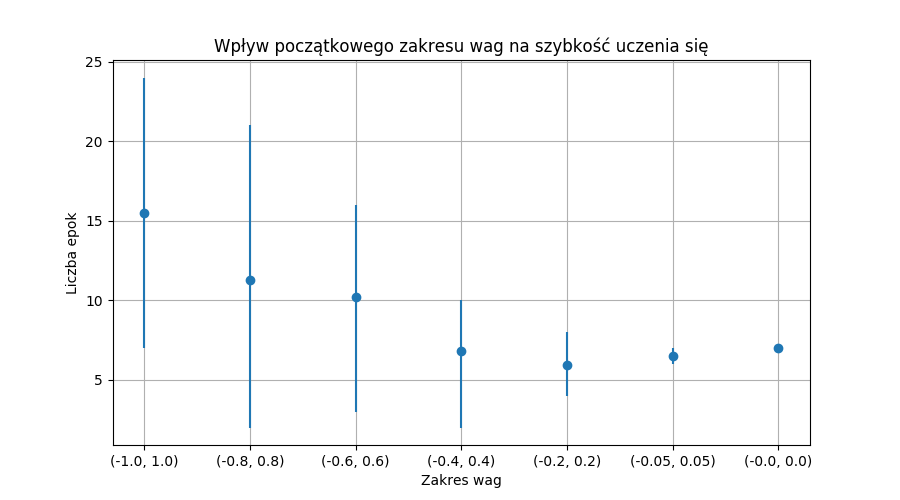
\includegraphics[scale=0.7]{test_weights_SimplePerceptron_10}
    \caption{Wyniki badań uzyskane w skutek 10 uruchomień}
    \end{figure}

    \begin{figure}[H]
    \centering
    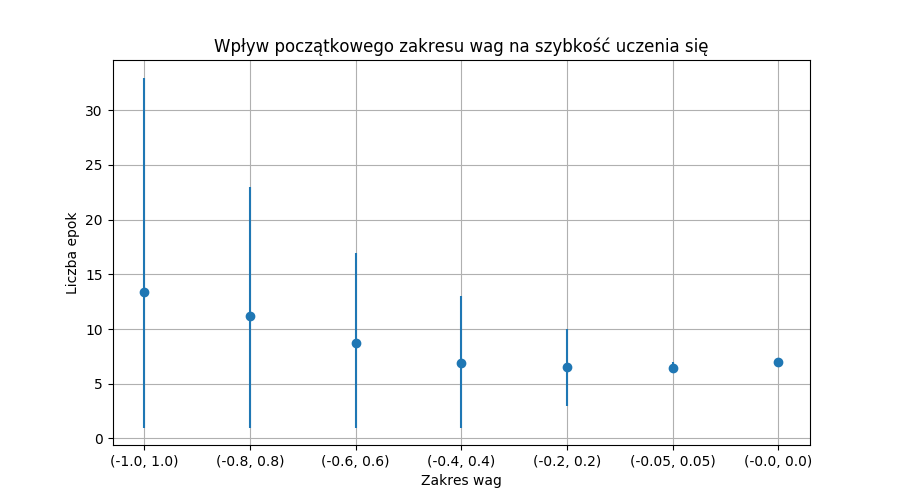
\includegraphics[scale=0.7]{test_weights_SimplePerceptron_100}
    \caption{Wyniki badań uzyskane w skutek 100 uruchomień}
    \end{figure}
    
    \paragraph{}
    W przeprowadzonych badaniach można zauważyć wzrost liczby epok wymaganych do dobrania odpowiednich wag, wraz ze wzrostem wielkości przedziału losowanych wag. Wynika to z faktu, że w przypadku dużych przedziałów wag mogą one wylosować skrajnie różne wartości. Duża różnica między początkową, a optymalną wartością wagi prowadzi, przy stałym współczynniku uczenia, do wzrostu wymaganej liczby epok, a co za tym idzie czasu wymaganego na ukończenie treningu.
    
    \paragraph{}
    Dalsze badanifffa ujawniły 
    
%     \begin{figure}
% \centering
% \begin{subfigure}{.5\textwidth}
%   \centering
%   \includegraphics[width=.4\linewidth]{image1}
%   \caption{A subfigure}
%   \label{fig:sub1}
% \end{subfigure}%
% \begin{subfigure}{.5\textwidth}
%   \centering
%   \includegraphics[width=.4\linewidth]{image1}
%   \caption{A subfigure}
%   \label{fig:sub2}
% \end{subfigure}
% \caption{A figure with two subfigures}
% \label{fig:test}
% \end{figure}
    
    
\end{document}
